\documentclass[conference,a4paper]{IEEEtran}

\usepackage[T1]{fontenc}
\usepackage[utf8]{inputenc}
\usepackage{microtype}
\usepackage{amsmath,amssymb}
\usepackage{graphicx}
\usepackage[caption=false,font=footnotesize]{subfig}
\usepackage{booktabs}
\usepackage{tikz}
\usetikzlibrary{arrows.meta,positioning,calc}
\usepackage{pgfplots}
\pgfplotsset{compat=1.17}
\usepackage{xcolor}
\usepackage{cite}
\usepackage{balance}
\usepackage[hidelinks]{hyperref}

\graphicspath{{../figures/}}

% Same palette as the full report.
\definecolor{ink}{HTML}{1B2A3A}
\definecolor{accent}{HTML}{0B6E8E}
\definecolor{cA}{HTML}{0072B2}
\definecolor{cB}{HTML}{D55E00}
\definecolor{cC}{HTML}{009E73}
\definecolor{cD}{HTML}{7F7F7F}
\colorlet{panel}{accent!7}

\tikzset{
  >={Stealth[length=1.6mm]},
  every picture/.style={line width=0.45pt, draw=ink, text=ink},
  box/.style={draw=ink, fill=panel, rounded corners=1.2pt, align=center,
              minimum height=6.5mm, inner sep=2.5pt, font=\scriptsize},
  ext/.style={box, fill=white, dashed},
  note/.style={font=\tiny, text=ink!85, align=center},
}
\pgfplotsset{
  paper/.style={
    width=\linewidth, height=0.62\linewidth,
    axis line style={draw=ink}, tick style={draw=ink},
    tick label style={font=\scriptsize}, label style={font=\scriptsize},
    legend style={font=\scriptsize, draw=none, fill=none, at={(0.5,1.03)}, anchor=south,
                  legend columns=-1, /tikz/every even column/.append style={column sep=6pt}},
    legend cell align=left, grid=major, grid style={draw=ink!12}, axis lines*=left,
  }
}

\newcommand{\unit}[1]{\ensuremath{\,\mathrm{#1}}}
\newcommand{\vect}[1]{\mathbf{#1}}

% Plan of the mission arena in metres, for use inside a tikzpicture whose x and y units are
% set to the wanted scale. Dimensions mirror src/trident_gazebo/worlds/arena.sdf.xacro.
\newcommand{\arenaplan}{%
  % floor and walls
  \fill[white] (-0.3,-0.6) rectangle (3.3,1.8);
  \draw[draw=ink, line width=1.1pt] (-0.3,-0.6) rectangle (3.3,1.8);
  \draw[draw=ink, line width=1.1pt] (0.9,-0.6) -- (0.9,0.2);
  \draw[draw=ink, line width=1.1pt] (0.9,1.0) -- (0.9,1.8);
  % entry line and start square
  \draw[draw=black, line width=0.9pt] (0,0) -- (0.15,0) arc (-90:-30:0.6) arc (150:90:0.6) -- (1.46,0.6);
  \fill[black] (1.40,0.54) rectangle (1.52,0.66);
  % pick bays: stem, crossbar, QR placard on the left wall
  \foreach \bx in {1.5,2.0,2.5} {
    \draw[draw=black, line width=0.9pt] (\bx,1.15) -- (\bx,1.45);
    \draw[draw=black, line width=0.9pt] (\bx-0.06,1.45) -- (\bx+0.06,1.45);
    \draw[draw=ink, line width=1.6pt] (\bx-0.08,1.79) -- (\bx+0.08,1.79);
  }
  % drop zones: stem, square, QR placard on the front wall
  \foreach \dy in {0.7,0.2,-0.3} {
    \draw[draw=black, line width=0.9pt] (2.575,\dy) -- (2.875,\dy);
    \fill[black!80] (2.875,\dy-0.125) rectangle (3.125,\dy+0.125);
    \draw[draw=ink, line width=1.6pt] (3.29,\dy-0.08) -- (3.29,\dy+0.08);
  }
}
% Coins in their bays, in the colour order of the default launch (red, green, blue)
\newcommand{\arenacoins}{%
  \fill[cB] (1.5,1.58) circle (0.02);
  \fill[cC] (2.0,1.58) circle (0.02);
  \fill[cA] (2.5,1.58) circle (0.02);
}
% Obstacle boxes of a preset: \arenaobstacles{1.90/0.55, 1.75/-0.15}
\newcommand{\arenaobstacles}[1]{%
  \foreach \ox/\oy in {#1} {
    \draw[draw=cB, fill=cB!35] (\ox-0.05,\oy-0.05) rectangle (\ox+0.05,\oy+0.05);
  }
}


\begin{document}

\title{Trident: Design and Simulation of a\\Differential-Drive Pick and Place Robot}

\author{\IEEEauthorblockN{Joshua John Leo Valan Johnson}
\IEEEauthorblockA{Roll No.\ 110123044\\
National Institute of Technology Tiruchirappalli, India}}

\maketitle

\begin{abstract}
Trident is a small differential-drive robot that I designed and built for a competition
task: follow a line, then carry coloured coins to the bins of their colours. This paper
reports its mechanical design and a simulation in which the whole task runs autonomously.
The gripper does not lift: two parabolic jaws on a pair of equal involute gears, driven by
one servo, cage a coin on the floor and the robot slides it, and a sliding condition for the
jaw profile is derived as a design rule. The mass properties of the CAD model show that the
centre of mass lies inside the support triangle but that the wheels carry only 18\,\% of
the weight, which limits the acceleration to 1.8\unit{m/s^2} and leaves a tipping margin of
a factor of two. The depth camera cannot see the last 0.15\unit{m} of floor, so an
eight-channel infrared array guides the end of every approach, on floor markings
dimensioned from its pitch. The robot is modelled in Gazebo from the CAD export, with
RTAB-Map and Nav2 for mapping and navigation and a line follower whose damping is shown to
be set by the distance of the array ahead of the axle. In twelve simulated missions with
four obstacle layouts the robot delivered all 36 coins, in 300\unit{s} per mission on
average, scored by a referee on ground truth. The line was followed within 6\unit{mm}, the
pose in the map was accurate to 10\unit{mm} RMS, and coins were placed within 21\unit{mm} of
the centres of their squares. All measurements were taken in simulation.
\end{abstract}

\begin{IEEEkeywords}
mobile robot design, differential drive, caging gripper, line following, visual SLAM,
navigation, Gazebo
\end{IEEEkeywords}

% ======================================================================================
\section{Introduction}
Trident is a small differential-drive robot that I designed and built for a task of the
WorldSkills competition: follow a black line, then carry plastic coins, cylinders about
40\unit{mm} across and 15\unit{mm} high, each to the bin of its colour. A first version was
a test rig for sensors and for ROS~2. The second, the subject of this paper, was designed in
SolidWorks, printed, and completed with its electronics in fifteen days
(\figurename~\ref{fig:teaser}). It won the district round. In the state round its infrared
array stopped working and the task was not completed.

A robot of this size has little room for mechanism, and one built in two weeks has little
time for trial runs. The work reported here therefore had two aims: a chassis, drive and
gripper that move a coin of known size with one servo and no sensing in the jaws, and a
simulation, built from the same CAD model, in which the whole mission can be run, scored
against ground truth and repeated.

The contributions are:
\begin{itemize}
  \item the mechanical design of the robot and of a gripper that cages a coin between two
        geared jaws and slides it along the floor (Section~\ref{sec:mech});
  \item an analysis of the design from the mass properties of the CAD model, which gives
        the wheel loads and the traction and tipping limits (Section~\ref{sec:mass});
  \item a Gazebo model of the robot with an emulated infrared array, and an arena whose
        floor markings are dimensioned from the pitch of that array
        (Sections~\ref{sec:sim} and~\ref{sec:arena});
  \item an autonomy stack in which a line follower takes over from the navigation where the
        camera can no longer see the floor (Section~\ref{sec:auto});
  \item measurements of the simulated mission over repeated runs
        (Section~\ref{sec:res}).
\end{itemize}
I am the sole author of the design, the hardware and the software.

\begin{figure*}[t]
  \centering
  \subfloat[CAD model]{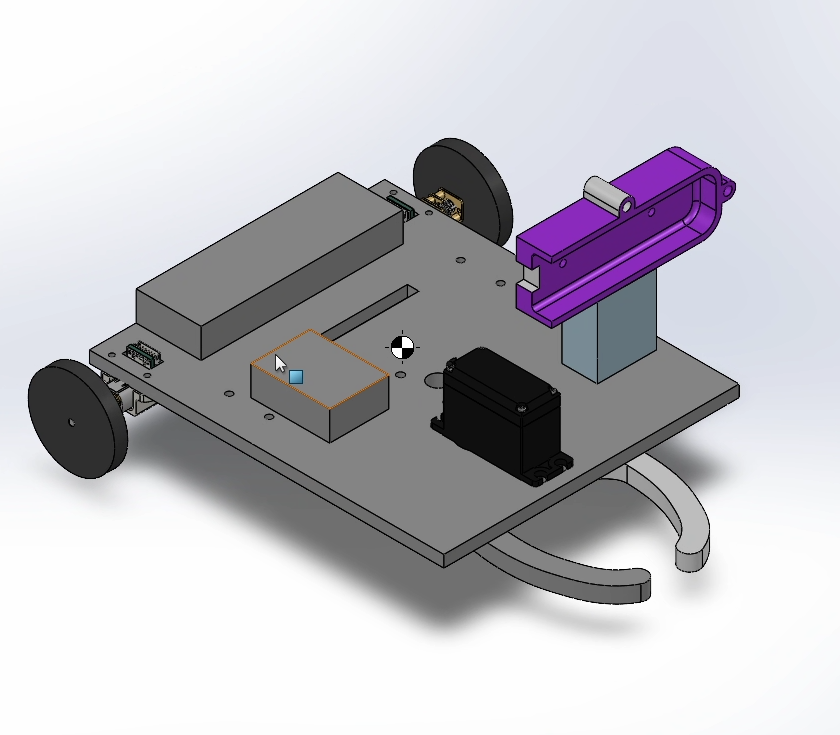
\includegraphics[height=3.6cm]{cad_iso.png}}\hfill
  \subfloat[Printed robot during wiring]{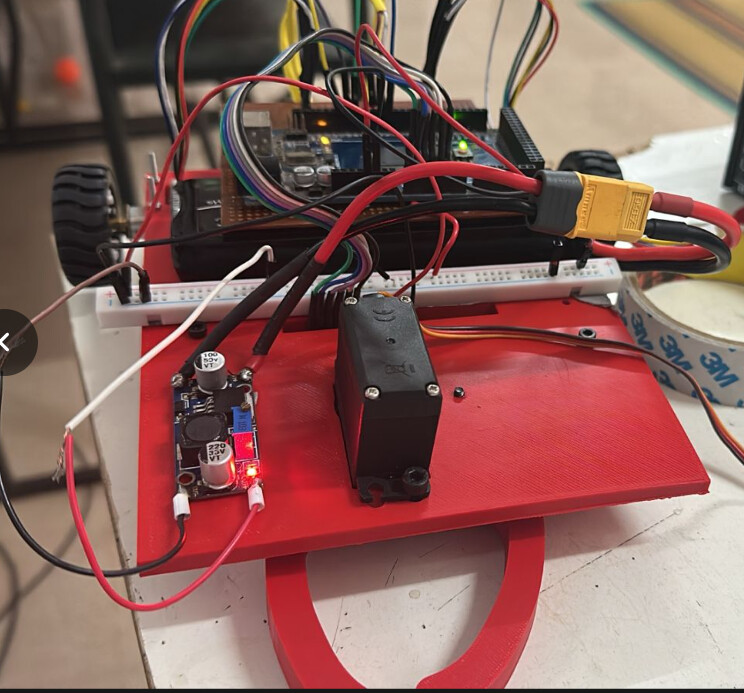
\includegraphics[height=3.6cm]{v2_hardware.jpg}}\hfill
  \subfloat[Simulated robot in the arena]{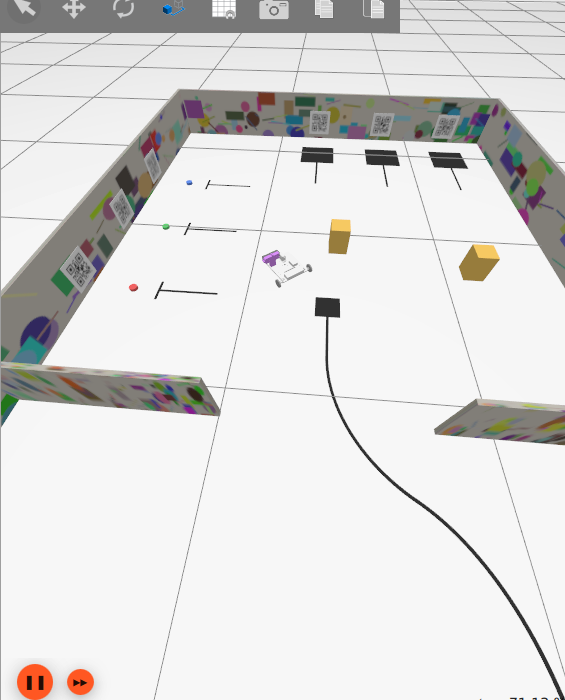
\includegraphics[height=3.6cm]{sim_arena.png}}
  \caption{Trident: two driven wheels at the rear, a ball caster under the plate and two
  geared jaws at the front. The holder at the side of the plate carries the depth camera.}
  \label{fig:teaser}
\end{figure*}

% ======================================================================================
\section{Related Work}
The kinematics and odometry of the differential drive are textbook material~\cite{siegwart},
and its frames in ROS are fixed by REP~105~\cite{rep105}. A line is commonly followed with a
proportional and derivative law~\cite{astrom} on the offset measured by a row of reflectance
sensors; the distance of the row ahead of the axle acts as the look-ahead of pure
pursuit~\cite{purepursuit}. A gripper that surrounds an object without clamping it is a
cage~\cite{caging}, and the sliding of a pushed object along its pusher was analysed by
Mason~\cite{mason}. The simulation uses Gazebo~\cite{gazebo} with ROS~2~\cite{ros2}. For
autonomy, RTAB-Map~\cite{rtabmap} provides visual SLAM on the streams of a RealSense depth
camera~\cite{realsense}, \texttt{robot\_localization}~\cite{robotlocalization} the odometry
filter, and Nav2~\cite{nav2} layered costmaps~\cite{costmap}, a
Dijkstra~\cite{dijkstra} planner and the Regulated Pure Pursuit controller~\cite{rpp},
sequenced by a behaviour tree~\cite{behaviortrees}. None of these components is new. The
contribution is the design of a robot around a task and the way its limits decide how the
components are combined.

% ======================================================================================
\section{Mechanical Design}
\label{sec:mech}
\subsection{Layout}
The chassis is one printed plate of $180\times150\times6\unit{mm}$. Two N20 gearmotors under
its rear edge drive wheels of 22\unit{mm} radius, 195.5\unit{mm} apart, and a ball caster
85\unit{mm} ahead of the axle is the third support. N20 motors were chosen because motors of
higher torque do not fit a robot of this size. The servo of the gripper stands on the plate
near its front edge, and the jaws turn in a horizontal plane below the plate. An array of
eight infrared reflectance channels at a pitch of 15\unit{mm} hangs under the plate,
48\unit{mm} ahead of the axle and 7.4\unit{mm} above the floor. An Intel RealSense D435
depth camera sits in a holder 85\unit{mm} above the floor and 54\unit{mm} to the left of the
centre line. All parts are printed in PLA; the chassis went through more than four printed
iterations to settle the tolerances for the bolts and nuts in use.

\subsection{Mass properties}
\label{sec:mass}
The design required the centre of mass to lie inside the support triangle of the wheels and
the caster. The CAD export gives the mass and centre of mass of every part, so this can be
checked and the wheel loads calculated. The model has a mass of
0.64\unit{kg}, and its centre of mass lies $x_c=69.3\unit{mm}$ ahead of the axle and
7.8\unit{mm} to the left (\figurename~\ref{fig:triangle}). With the caster at
$x_k=85.0\unit{mm}$ and $W=6.28\unit{N}$, the static loads on the caster and on the two
wheels together are
\begin{equation}
  N_k = W\frac{x_c}{x_k} = 5.12\unit{N}, \qquad N_w = W\Bigl(1-\frac{x_c}{x_k}\Bigr) = 1.16\unit{N}.
  \label{eq:loads}
\end{equation}
The centre of mass is inside the triangle, as required, and lies closer to the caster than
to the axle: the wheels carry 18\,\% of the weight.
The camera and its holder, 131\unit{g} at the front of the plate, are the main cause. Three
consequences follow.

\emph{Traction.} With a friction coefficient $\mu$ the wheels can accelerate or brake the
robot at no more than
\begin{equation}
  a_{\max} = \mu g\Bigl(1-\frac{x_c}{x_k}\Bigr) = 1.8\,\mu\unit{m/s^2}.
  \label{eq:traction}
\end{equation}
In the simulation, a robot without a braking limit skidded and turned on every stop
command; the drive is now limited to 1.0\unit{m/s^2}.

\emph{Drive sizing.} On the motor data assumed in the model (300\unit{rpm}, 0.05\unit{N\,m}
at the wheel, both placeholders) the motors can push with 4.5\unit{N} at stall, four times
what the wheels can transmit. The drive is limited by traction and not by torque.

\emph{Tipping.} The triangle is narrow at the caster. The centre of mass is 6.7\unit{mm}
from its left edge and 42\unit{mm} above the floor, so a braking deceleration above
2.1\unit{m/s^2} tips the robot over that edge. The margin over the allowed 1.0\unit{m/s^2}
is a factor of two.

Moving the caster forward and the camera to the centre line would correct all three. The
masses are CAD values and the printed robot has not been weighed on its supports, so the
real centre of mass may lie further back.

\begin{figure}[t]
  \centering
  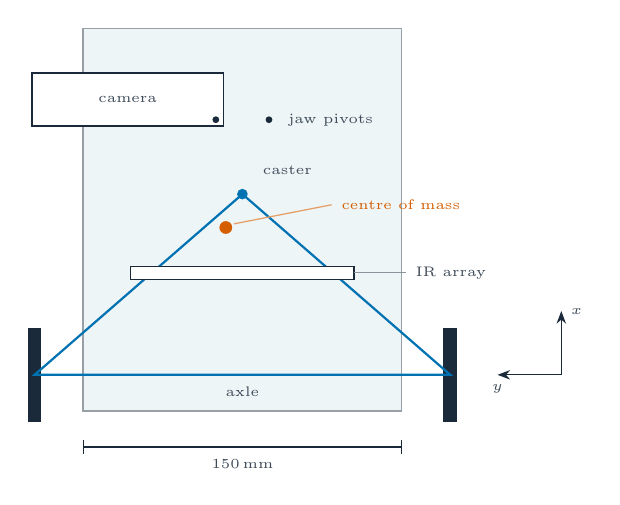
\begin{tikzpicture}[scale=0.27]
    \draw[draw=ink!45, fill=panel] (-7.5,-1.7) rectangle (7.5,16.3);
    \fill[ink] (-10.1,-2.2) rectangle (-9.45,2.2);
    \fill[ink] (9.45,-2.2) rectangle (10.1,2.2);
    \draw[cA, line width=0.8pt] (-9.777,0) -- (9.777,0) -- (0,8.5) -- cycle;
    \fill[cA] (0,8.5) circle (0.25);
    \node[note, anchor=west] at (0.5,9.6) {caster};
    \node[note, anchor=north] at (0,-0.1) {axle};
    \fill[cB] (-0.78,6.93) circle (0.3);
    \draw[draw=cB!60] (-0.4,7.1) -- (4.2,8.0);
    \node[note, anchor=west, text=cB] at (4.2,8.0) {centre of mass};
    \draw[draw=ink, fill=white] (-9.9,11.7) rectangle (-0.9,14.2);
    \node[note] at (-5.4,12.95) {camera};
    \fill[ink] (-1.25,12.0) circle (0.16);
    \fill[ink] (1.25,12.0) circle (0.16);
    \node[note, anchor=west] at (1.7,12.0) {jaw pivots};
    \draw[draw=ink, fill=white] (-5.25,4.5) rectangle (5.25,5.1);
    \node[note, anchor=west] at (7.7,4.8) {IR array};
    \draw[draw=ink!50] (5.25,4.8) -- (7.7,4.8);
    \draw[->] (15,0) -- (15,3) node[note, right] {$x$};
    \draw[->] (15,0) -- (12,0) node[note, below] {$y$};
    \draw[|-|] (-7.5,-3.4) -- (7.5,-3.4);
    \node[note, below] at (0,-3.5) {150\,mm};
  \end{tikzpicture}
  \caption{Support triangle of the wheels and the caster from above, to scale. The centre of
  mass of the model is 16\unit{mm} behind the caster and 6.7\unit{mm} from the left edge.}
  \label{fig:triangle}
\end{figure}

\subsection{Gripper}
The robot is light, and a coin held out in front of the caster could tip it forward. The
gripper therefore does not lift. Two jaws close around the coin on the floor and the robot
slides it to its destination; it is enough that the coin cannot leave the space between the
jaws (\figurename~\ref{fig:gripper}). This removes the lift axis and the need to know the
mass of the coin.

The jaws have a parabolic profile, so that a coin which meets a jaw anywhere along its
length is led inward. For a profile $y^2=4fx$ that advances along its axis onto a coin at a
lateral offset $y$, the surface at the contact is inclined at $\tan\alpha=2f/y$ to the
direction of travel. The coin slides along the jaw as long as the direction of travel lies
outside the friction cone about the surface normal, $90^\circ-\alpha>\arctan\mu$, that is,
\begin{equation}
  \lvert y\rvert > 2\mu f .
  \label{eq:centring}
\end{equation}
Centring therefore works best at the tips of the jaws, where a misaligned approach makes
first contact, and improves with a short focal length and a slippery jaw. The focal length
of the printed jaws was not measured, and \eqref{eq:centring} is a design rule and not a
verified figure.

Each jaw carries a ridge near its pivot. When the jaws open, the ridges push the coin out,
so that it is not drawn back with the robot. One MG995 servo turns one jaw directly, and a
pair of involute gears~\cite{shigley} with equal numbers of teeth, on pivots 25\unit{mm}
apart, turns the other by the same angle in the opposite sense. The stall torque of
0.83\unit{N\,m} gives 9\unit{N} at the tip of a jaw 90\unit{mm} long, against the
0.08\unit{N} that slides a coin of 23\unit{g}.

\begin{figure}[t]
  \centering
  \subfloat[Jaws and gear pair]{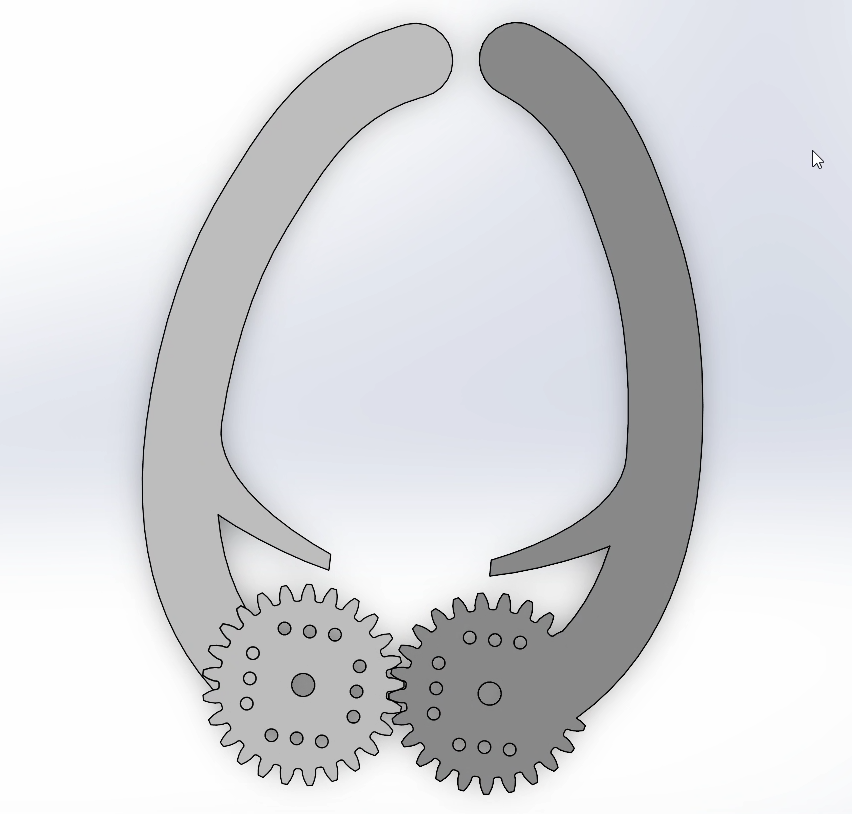
\includegraphics[height=3.0cm]{gripper_cad.png}}\hfill
  \subfloat[Coin against a parabolic jaw]{%
    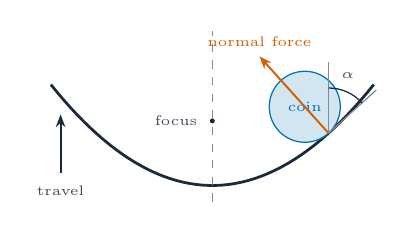
\begin{tikzpicture}[scale=0.82]
      \draw[ink, line width=1.0pt, domain=-2.5:2.5, samples=50] plot (\x,{\x*\x/4});
      \draw[dashed, draw=ink!55] (0,-0.25) -- (0,2.4);
      \fill[ink] (0,1) circle (1.1pt);
      \node[note, anchor=east] at (-0.08,1.0) {focus};
      \coordinate (P) at (1.8,0.81);
      \draw[draw=cA, fill=cA!18] ($(P)+(-0.368,0.409)$) circle (0.55);
      \node[note, text=cA] at ($(P)+(-0.368,0.409)$) {coin};
      \draw[->, cB, line width=0.7pt] (P) -- ($(P)+(-1.07,1.19)$);
      \node[note, text=cB, anchor=south] at ($(P)+(-1.07,1.19)$) {normal force};
      \draw[draw=ink!55] (P) -- ($(P)+(0.74,0.67)$);
      \draw[draw=ink!55] (P) -- ($(P)+(0,1.1)$);
      \draw[draw=ink] ($(P)+(0,0.7)$) arc (90:42:0.7);
      \node[note] at ($(P)+(0.3,0.9)$) {$\alpha$};
      \draw[->, line width=0.7pt] (-2.35,0.2) -- (-2.35,1.1);
      \node[note, anchor=north] at (-2.35,0.15) {travel};
    \end{tikzpicture}}
  \caption{The gripper. A coin is pushed along the normal of the profile, which has an
  inward component everywhere except at the vertex.}
  \label{fig:gripper}
\end{figure}

\subsection{What the camera cannot see}
The depth image has a vertical field of view of $58^\circ$. From a height of 85\unit{mm} its
lowest ray reaches the floor at $85\unit{mm}/\tan 29^\circ\approx0.15\unit{m}$ ahead of the
lens, and depth is not reported below 0.2\unit{m}. A caged coin lies about 4\unit{cm} ahead
of the lens. The camera therefore never sees the coin that the robot is about to pick, nor
the last 15\unit{cm} of floor. This is the most important constraint that the mechanical
design places on the software.

% ======================================================================================
\section{Simulation Model}
\label{sec:sim}
The robot is simulated in Gazebo Fortress with ROS~2 Humble, in an unprivileged Docker
container. The robot description is maintained by hand on top of the URDF export of the CAD
assembly. The export needed corrections before it was usable: a floor frame after
REP~105, wheel axes turned so that positive rotation drives forward, a right wheel that
the export had placed 0.5\unit{mm} off the axle, gripper joint limits that were all zero,
the body of the camera, which was missing from the assembly, and a mass for the infrared
array. The chassis mesh of 277\,864 triangles is replaced for contact by boxes, cylinders
and a sphere; the jaws keep their meshes, since their shape is what the gripper depends on.
Gazebo Fortress ignores the mimic relation of a URDF, so the gear pair is reproduced by a
node that sends the commanded angle to one jaw and its negative to the other.

The depth camera is modelled with the field of view of the D435, $87^\circ\times58^\circ$,
at $848\times480$ pixels. Gazebo has no reflectance sensor, so each infrared channel is a
camera of $8\times8$ pixels that looks down on a spot about 8\unit{mm} across. A node
averages each image into a voltage between 0 and 5\unit{V} and adds Gaussian noise of
0.05\unit{V}. A channel over the edge of a line returns an intermediate voltage, as the
real sensor does. The arena is lit evenly and without shadows, so that the readings do not
depend on heading. Motors and servo are ideal within their limits, and the floor is flat.

% ======================================================================================
\section{Arena}
\label{sec:arena}
The arena models the structure of the task and does not reproduce the competition field
(\figurename~\ref{fig:arena}). It measures $3.6\times2.4\unit{m}$. A line leads from the
start through an S-bend and a doorway to a start square in a room with three pick bays on
one wall and three drop zones on another. A QR code behind each station names a colour: of
the coin at a bay, of the coins accepted at a drop zone. The assignment is a launch argument,
as is one of three layouts of obstacle boxes.

The floor markings follow from the pitch $p=15\unit{mm}$ and the span of 105\unit{mm} of the
infrared array. Lines are 12\unit{mm} wide, less than one pitch, so that a line darkens at
most two neighbouring channels, each partially, and its position can be interpolated.
Markers (the start square and the crossbars of the bays) are 120\unit{mm} wide, more than
the span, so that all eight channels go dark together, which nothing else on the floor can
cause. A pick bay is a T: a stem of 0.30\unit{m} leads to a crossbar, and the coin lies
0.13\unit{m} beyond it, the distance from the array to the space between the open jaws. A
drop zone is a stem into a square of 250\unit{mm}. The walls carry generated textures,
because plain walls give a visual SLAM system nothing to track.

% ======================================================================================
\section{Autonomy}
\label{sec:auto}
Odometry, mapping, localisation and navigation are existing packages configured for this
robot; the line follower, the docking sequences, the mission state machine and the referee
were written for it (\figurename~\ref{fig:arch}).

\begin{figure}[t]
  \centering
  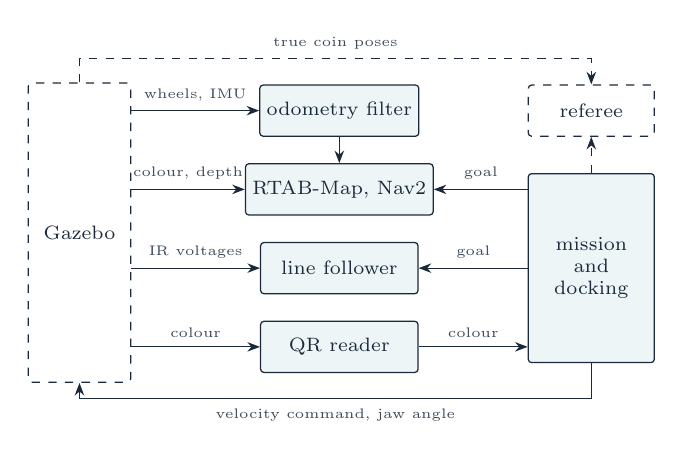
\begin{tikzpicture}
    \node[ext, minimum width=13mm, minimum height=38mm] (sim) at (0,0) {Gazebo};
    \node[box, minimum width=20mm] (ekf) at (3.3,1.55) {odometry filter};
    \node[box, minimum width=20mm] (slam) at (3.3,0.55) {RTAB-Map, Nav2};
    \node[box, minimum width=20mm] (line) at (3.3,-0.45) {line follower};
    \node[box, minimum width=20mm] (qr) at (3.3,-1.45) {QR reader};
    \node[box, minimum width=16mm, minimum height=24mm] (mis) at (6.5,-0.45) {mission\\and\\docking};
    \node[ext, minimum width=16mm] (ref) at (6.5,1.55) {referee};
    \draw[->] (sim.east |- ekf) -- node[note, above] {wheels, IMU} (ekf);
    \draw[->] (sim.east |- slam) -- node[note, above] {colour, depth} (slam);
    \draw[->] (sim.east |- line) -- node[note, above] {IR voltages} (line);
    \draw[->] (sim.east |- qr) -- node[note, above] {colour} (qr);
    \draw[->] (ekf) -- (slam);
    \draw[->] (mis.west |- slam) -- node[note, above] {goal} (slam);
    \draw[->] (mis.west |- line) -- node[note, above] {goal} (line);
    \draw[->] (qr) -- node[note, above] {colour} (mis.west |- qr);
    \draw[->, dashed] (mis) -- (ref);
    \draw[->] (mis.south) -- ++(0,-0.45) -| node[note, pos=0.25, below] {velocity command, jaw angle} (sim.south);
    \draw[->, dashed] (sim.north) -- ++(0,0.3) -| node[note, pos=0.25, above] {true coin poses} (ref.north);
  \end{tikzpicture}
  \caption{Software architecture. Dashed boxes exist only in simulation.}
  \label{fig:arch}
\end{figure}

\subsection{Localisation and navigation}
An extended Kalman filter fuses the forward speed of the wheels with the yaw rate of the
gyroscope; the yaw rate of the wheels is left out because they slip when the robot turns on
the spot. RTAB-Map builds the map once, on a survey of the empty arena with a full turn at
each of seven stops, and localises in it during a mission. Nav2 plans with NavFn on a costmap
of 2\unit{cm} cells, replans once a second, and tracks the path at 0.15\unit{m/s}. Obstacles
come from the depth image between 3\unit{cm} and 0.40\unit{m} above the floor. Because the
camera looks forward only, the controller may not reverse and the back-up recovery is
removed from the behaviour tree.

The arena shows each QR code twice, at a bay and at a drop zone. Seen from close by, a
match of the features of the code alone made RTAB-Map place the robot in front of the other
wall. A fix is therefore accepted only when its matched features are spread across the
image; during development true views scored 0.004 to 0.014 on this measure and look-alikes
below 0.0025, and the threshold is 0.005.

\subsection{Line follower}
Each voltage is converted to a darkness $d_i$ between 0 and 1, with readings below 0.15 set
to zero. The line offset is the weighted mean $e=p\sum_i d_i(i-3.5)/\sum_i d_i$, and the
robot steers with
\begin{equation}
  \omega = \operatorname{sat}_{\omega_{\max}}\bigl(k_p e + k_d\dot e\bigr),
  \label{eq:steer}
\end{equation}
with $k_p=45\unit{rad/(s\,m)}$, $k_d=2\unit{rad/m}$ and $\omega_{\max}=1.5\unit{rad/s}$ at
20\unit{Hz}. Let the array be a distance $L$ ahead of the axle, $\psi$ the heading relative
to the line and $y=-e$ the lateral position of the array. Then $\dot y=v\psi+L\omega$ and
$\dot\psi=\omega$, and with the proportional part of \eqref{eq:steer},
\begin{equation}
  \ddot y + Lk_p\,\dot y + vk_p\,y = 0 ,
\end{equation}
with damping ratio $\zeta=\tfrac12 L\sqrt{k_p/v}$. The damping comes entirely from $L$: an
array on the axle would oscillate under proportional control at any gain. With
$L=48\unit{mm}$, $\zeta$ is 0.51 at the entry speed of 0.10\unit{m/s} and 0.72 at the
docking speed of 0.05\unit{m/s}. A marker is reported when six or more channels are dark in
two successive samples.

\subsection{Docking and mission}
Nav2 brings the robot to a station pose on the extension of a stem, about 0.15\unit{m}
short of its foot. The line follower then drives until the array finds the stem, steers
onto it and stops at the marker. To pick, the robot opens the jaws, follows the stem to the
crossbar, reads the QR code, closes the jaws and backs out by the distance just driven. To
drop, it follows the stem until the array enters the square, opens the jaws and backs out.
The stem absorbs the error of the navigation, and backing out along a path just driven
needs no sensing behind the robot. A QR code is trusted only at its station and after three
identical decodes, since the decoder does not report where in the image a code lies.

The mission follows the entry line, reads the three drop zones, then picks and delivers the
three coins. A station whose marker is not found is tried once more; a coin whose code
cannot be read is left in its bay. A referee reads the true positions of the coins from the
simulator and passes a run when every coin lies inside the square of its colour. Nothing on
the robot may read the ground truth.

% ======================================================================================
\section{Results}
\label{sec:res}
The mission was run twelve times without a display, three runs for each obstacle layout
(none and three presets of two or three boxes), with eleven different combinations of pick
and drop colours, the same map and the same start pose. A recording node that only listens
logged the true pose, the pose in the map and the odometry at 10\unit{Hz}.

All twelve runs passed, with 36 coins of 36 inside the squares of their colours
(Table~\ref{tab:res}). No station needed a second attempt and the navigation entered no
recovery. A mission takes 300\unit{s} on average: 19\unit{s} on the entry line,
83\unit{s} for the survey of the drop zones and 66\unit{s} per coin. The obstacles cost at
most 5\unit{s}. \figurename~\ref{fig:path} shows the true path of one run.

\begin{table}[t]
  \caption{Twelve simulated missions and 36 picks and drops}
  \label{tab:res}
  \centering\footnotesize
  \begin{tabular}{@{}lcc@{}}
    \toprule
    Quantity & Mean or RMS & Range or largest \\
    \midrule
    Coins delivered & 36 of 36 & \\
    Mission time & 300\unit{s} & 293 to 307\unit{s} \\
    Path length & 18.1\unit{m} & 17.5 to 18.7\unit{m} \\
    Offset from entry line (RMS) & 1.6\unit{mm} & 6.0\unit{mm} \\
    Map pose error (RMS) & 9.9\unit{mm} & 39\unit{mm} \\
    Map heading error (RMS) & $0.7^\circ$ & \\
    Odometry alone, error at end & 16\unit{mm} & 30\unit{mm} \\
    Pick: lateral offset on crossbar (RMS) & 2.7\unit{mm} & 7.1\unit{mm} \\
    Pick: heading error (RMS) & $2.9^\circ$ & $7.1^\circ$ \\
    Drop: coin from square centre & 9.0\unit{mm} & 20.7\unit{mm} \\
    \bottomrule
  \end{tabular}
\end{table}

\begin{figure}[t]
  \centering
  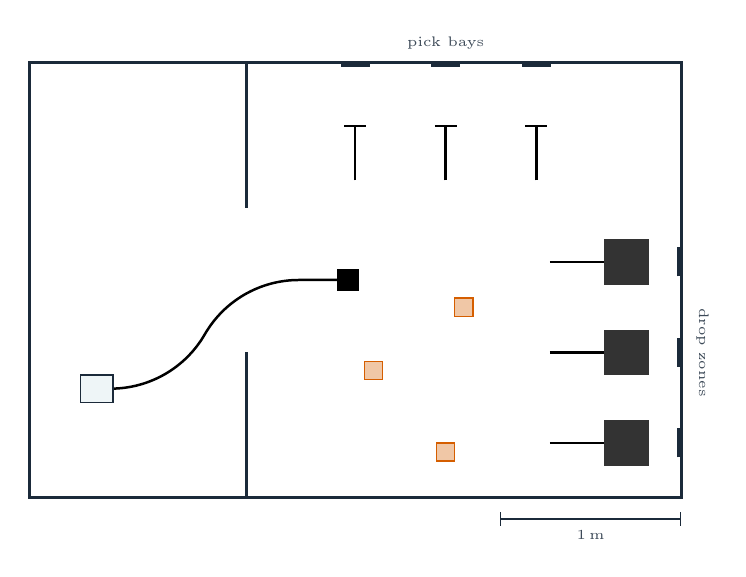
\begin{tikzpicture}[x=2.3cm, y=2.3cm]
    \arenaplan
    \arenaobstacles{2.10/0.45, 1.60/0.10, 2.00/-0.35}
    \draw[cA, line width=0.4pt, line join=round] plot file {../data/track_m03.dat};
    \draw[draw=ink, fill=panel] (-0.017,-0.075) rectangle (0.163,0.075);
    \node[note, anchor=south] at (2.0,1.82) {pick bays};
    \node[note, rotate=-90, anchor=south] at (3.33,0.2) {drop zones};
    \draw[|-|] (2.3,-0.72) -- (3.3,-0.72);
    \node[note, below] at (2.8,-0.73) {1\,m};
  \end{tikzpicture}
  \caption{Plan of the arena, to scale, with the true path of the robot in one mission
  with three obstacle boxes. The entry line leads from the start, at the left, to the start
  square in the room.}
  \label{fig:arena}\label{fig:path}
\end{figure}

\emph{Line following.} The array stayed within 6.0\unit{mm} of the line, a tenth of the
channel pitch in RMS terms, so the interpolation between partially covered channels works
as intended. Run alone on the entry line (\figurename~\ref{fig:line}), the follower is
insensitive to noise up to 0.2\unit{V}, four times the nominal level, and degrades above
it, when noise crosses the floor threshold. The offset grows quickly with speed, from
1.1\unit{mm} RMS at 0.05\unit{m/s} to 17.6\unit{mm} at 0.30\unit{m/s}, in the direction
that the fall of $\zeta$ from 0.72 to 0.29 predicts.

\begin{figure}[t]
  \centering
  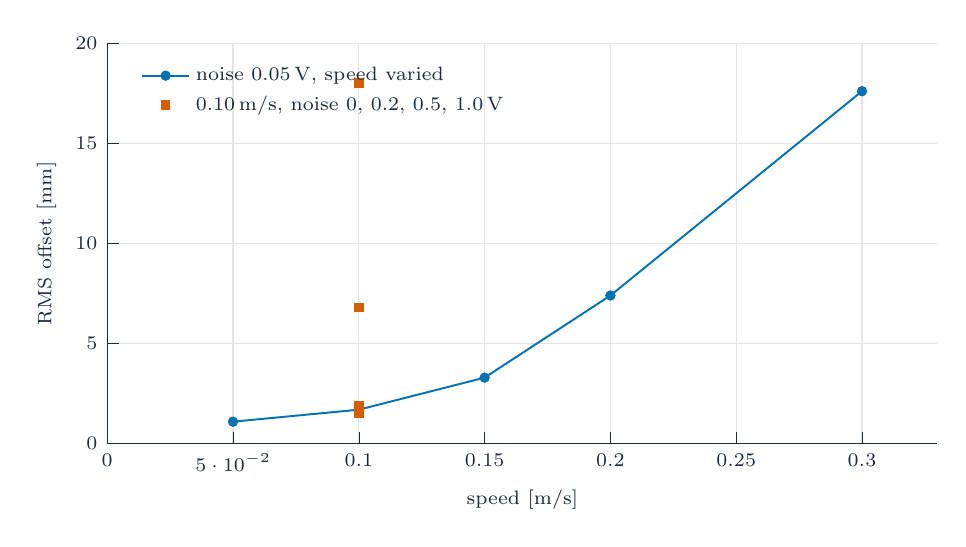
\begin{tikzpicture}
    \begin{axis}[paper, height=0.55\linewidth, xlabel={speed [m/s]}, ylabel={RMS offset [mm]},
        xmin=0, xmax=0.33, ymin=0, ymax=20, legend columns=1,
        legend style={at={(0.03,0.97)}, anchor=north west}]
      \addplot[cA, mark=*, mark size=1.5pt, line width=0.7pt] coordinates
        {(0.05,1.1) (0.10,1.7) (0.15,3.3) (0.20,7.4) (0.30,17.6)};
      \addplot[only marks, mark=square*, mark size=1.5pt, cB] coordinates
        {(0.10,1.5) (0.10,1.9) (0.10,6.8) (0.10,18.0)};
      \legend{{noise 0.05\,V, speed varied},{0.10\,m/s, noise 0, 0.2, 0.5, 1.0\,V}}
    \end{axis}
  \end{tikzpicture}
  \caption{Line follower alone on the entry line, one run per point: RMS offset of the array
  from the line.}
  \label{fig:line}
\end{figure}

\emph{Localisation.} The pose in the map was within 9.9\unit{mm} RMS of the truth. The
odometry filter alone, however, was never more than 30\unit{mm} off in any run: the
simulated encoders are ideal and the floor is uniform. The runs show that the localisation
is stable and does not jump; they do not show what it would contribute on a real floor.

\emph{Docking.} When the jaws closed, the array was 2.7\unit{mm} RMS to the side of the
stem and always on the crossbar. Heading is the least well controlled quantity, with
$7.1^\circ$ at worst, and all 36 coins were nevertheless caged, which is the tolerance that
the shape of the jaws was meant to provide. Released coins lay 9.0\unit{mm} from the centre
of a square that extends 125\unit{mm} from it.

% ======================================================================================
\section{Limitations}
All measurements were taken in simulation, and none on the printed robot. The masses are
CAD values and the motor data placeholders; the robot was not weighed. The simulated motors
are ideal within their limits and the encoders have no quantisation, so the odometry is
better than it would be on a floor. The arena was designed with the software: its markings,
wall textures and shadow-free lighting are the conditions under which the approach works.
The twelve runs share one map and one start pose, and each line-following condition was run
once. The condition that rejects look-alike views is one number chosen for this arena. The
planner treats the robot as a disc that does not enclose the jaws. The mission has no
feedback from the jaws, and, like the robot that failed in the state round, it depends on a
single line sensor with no fallback.

% ======================================================================================
\section{Conclusion}
The design decisions that matter most in Trident are the ones that removed something: a
gripper without a lift axis or a sensor, and no second camera for the floor that the first
cannot see. Two lessons recur. A model answers questions that were settled by eye during
the build: the centre of mass lies inside the support triangle, as intended, but the CAD
model puts 82\,\% of the weight on the caster, which the simulation showed as a skid before the
calculation explained it. And the position of a sensor is a control parameter: the distance
of the infrared array ahead of the axle sets the damping of the line follower. The
simulated mission is complete and repeatable. The steps that remain are on the hardware: to
weigh the robot and move the caster and the camera, to replace the breadboard wiring, and to
run the mission on the printed robot.

\balance
\bibliographystyle{IEEEtran}
\bibliography{references}

\end{document}
